%===================================================================================
% JORNADA CIENTÍFICA ESTUDIANTIL - MATCOM, UH
%===================================================================================
% Esta plantilla ha sido diseñada para ser usada en los artículos de la
% Jornada Científica Estudiantil, MatCom.
%
% Por favor, siga las instrucciones de esta plantilla y rellene en las secciones
% correspondientes.
%
% NOTA: Necesitará el archivo 'jcematcom.sty' en la misma carpeta donde esté este
%       archivo para poder utilizar esta plantila.
%===================================================================================



%===================================================================================
% PREÁMBULO
%-----------------------------------------------------------------------------------
\documentclass[a4paper,10pt,twocolumn]{article}

%===================================================================================
% Paquetes
%-----------------------------------------------------------------------------------
\usepackage{amsmath}
\usepackage{amsfonts}
\usepackage{amssymb}
\usepackage{jcematcom}
\usepackage[utf8]{inputenc}
\usepackage{listings}
\usepackage[pdftex]{hyperref}
\usepackage[ruled,vlined,lined,linesnumbered]{algorithm2e}
\usepackage{xcolor} % para definir
\usepackage{pstricks} % para utilizar colores propios
%-----------------------------------------------------------------------------------
% Comandos
%-----------------------------------------------------------------------------------
\newcommand{\la}{\leftarrow}
\newcommand{\ra}{\rightarrow}
\newcommand{\ioi}{\Leftrightarrow}
\newcommand{\pred}[1]{{\rm pred}_{#1}} % antecesor
\newcommand{\predi}{\pred{i}} % antecesor en el nivel i
\newcommand{\idx}{{\rm idx}}
\newcommand{\fwd}[1]{{\rm forward}[#1]}
\newcommand{\fwdi}{\fwd{i}}
\newcommand{\withT}{{\rm width}}
\newcommand{\with}[1]{\withT[#1]}
\newcommand{\withi}{\with{i}}
\newcommand{\key}{{\rm key}}
\newcommand{\lev}{{\rm level}}
\newcommand{\nil}{{\rm NIL}}
\newcommand{\To}{{\bf to}}

%-----------------------------------------------------------------------------------
% Configuración
%-----------------------------------------------------------------------------------
\hypersetup{colorlinks,%
	    citecolor=black,%
	    filecolor=black,%
	    linkcolor=black,%
	    urlcolor=blue}

\definecolor{disliHeaderIdxColor}{RGB}{0, 176, 80}
\definecolor{disliNodeKeyColor}{RGB}{31, 78, 121}
\definecolor{disliNodeIdxColor}{RGB}{46, 117, 182}
\definecolor{disliNilReferenceColor}{RGB}{166, 166, 166}
\definecolor{disliWUpRef}{RGB}{112, 173, 71}

\newcommand{\disliHeaderIdxColor}[1]{{\color{disliHeaderIdxColor}#1}}
\newcommand{\disliNodeKeyColor}[1]{{\color{disliNodeKeyColor}#1}}
\newcommand{\disliNodeIdxColor}[1]{{\color{disliNodeIdxColor}#1}}
\newcommand{\disliNilReferenceColor}[1]{{\color{disliNilReferenceColor}#1}}
\newcommand{\disliWUpRef}[1]{{\color{disliWUpRef}#1}}
%===================================================================================



%===================================================================================
% Presentacion
%-----------------------------------------------------------------------------------
% Título
%-----------------------------------------------------------------------------------
\title{Documento de Ejemplo para la Jornada Científica Estudiantil}

%-----------------------------------------------------------------------------------
% Autores
%-----------------------------------------------------------------------------------
\author{\\
\name Andy Ledesma García \email \href{mailto:a.uno@lab.matcom.uh.cu}{a.uno@lab.matcom.uh.cu}
	\\ \addr Grupo C211 \AND
\name Omar Alejandro Hernández Ramírez \email \href{mailto:a.dos@lab.matcom.uh.cu}{a.dos@lab.matcom.uh.cu}
  \\ \addr Grupo C212}

%-----------------------------------------------------------------------------------
% Tutores
%-----------------------------------------------------------------------------------
\tutors{\\
Dr. Tutor Uno, \emph{Centro} \\
Lic. Tutor Dos, \emph{Centro}}

%-----------------------------------------------------------------------------------
% Headings
%-----------------------------------------------------------------------------------
\jcematcomheading{\the\year}{1-\pageref{end}}{A. Uno, A. Dos}

%-----------------------------------------------------------------------------------
\ShortHeadings{Ejemplo JCE}{Autores}
%===================================================================================



%===================================================================================
% DOCUMENTO
%-----------------------------------------------------------------------------------
\begin{document}

%-----------------------------------------------------------------------------------
% NO BORRAR ESTA LINEA!
%-----------------------------------------------------------------------------------
\twocolumn[
%-----------------------------------------------------------------------------------

\maketitle

%===================================================================================
% Resumen y Abstract
%-----------------------------------------------------------------------------------
\selectlanguage{spanish} % Para producir el documento en Español

%-----------------------------------------------------------------------------------
% Resumen en Español
%-----------------------------------------------------------------------------------
\begin{abstract}

	El Resumen en Español debe constar de $100$ a $200$ palabras y presentar de forma
	clara y concisa el contenido fundamental del artículo.

\end{abstract}

%-----------------------------------------------------------------------------------
% English Abstract
%-----------------------------------------------------------------------------------
\vspace{0.5cm}

\begin{enabstract}

  The English Abstract must have have $100$ to $200$ words, and present in a clear
  and concise form the essentials of the article content.

\end{enabstract}

%-----------------------------------------------------------------------------------
% Palabras clave
%-----------------------------------------------------------------------------------
\begin{keywords}
	Separadas,
	Por,
	Comas.
\end{keywords}

%-----------------------------------------------------------------------------------
% Temas
%-----------------------------------------------------------------------------------
\begin{topics}
	Tema, Subtema.
\end{topics}


%-----------------------------------------------------------------------------------
% NO BORRAR ESTAS LINEAS!
%-----------------------------------------------------------------------------------
\vspace{0.8cm}
]
%-----------------------------------------------------------------------------------


%===================================================================================

%===================================================================================
% Introducción
%-----------------------------------------------------------------------------------
\section{Introducción}\label{sec:intro}
%-----------------------------------------------------------------------------------
  El \textbf{P}roblema de \textbf{E}nrutamiento de \textbf{V}ehículos
  (\textbf{VRP} por sus siglas en inglés), es uno de los problemas de gestión más
  comunes en la distribución de bienes y servicios. Consiste en un conjunto de
  nodos (clientes) que deben ser visitados por un conjunto de entidades (vehículos).
  Una ruta se define como el recorrido que un vehículo realiza visitando un grupo de
  clientes en un orden específico. En el VRP pueden ser optimizadas distintas 
  funciones como el número de clientes atendidos, el costo total de los recorridos o 
  las unidades de la mercancía que se transporta.
  
  Este problema es NP-duro \cite{Paolo}, por lo tanto, para solucionar pequeñas 
  instancias del VRP se emplean métodos exactos, mientras que, para instancias mayores, 
  se recurre al uso de heurísticas y metaheurísticas.
  
  Una de las metaheurísticas que mejores resultados obtiene es \textbf{B}úsqueda de
  \textbf{V}ecindad \textbf{V}ariable \cite{Mla} (\textbf{VNS}, su acrónimo en inglés),
  particularmente, la variante IVNS \cite{Camila}.Esta estrategia consiste en elegir 
  una solución $ S $ y definir una estructura de entorno $ V $, para luego explorar las 
  soluciones ``vecinas'' de $ S $ en $ V $. En IVNS se consideran infinitas estructuras
  de entorno. Las nuevas soluciones se aceptan o rechazan en dependencia de su calidad 
  para el problema y el algoritmo en cuestión. Por ejemplo, en \textit{Recocido Simulado} 
  se aceptan soluciones peores en base a determinada probabilidad que depende de un 
  parámetro del algoritmo \cite{Alina}.
  
  Para obtener cada una de las nuevas soluciones, se le realizan cambios en una o varias
  rutas a $ S $, la solución inicial, como son \cite{Camila, Andy}:
  \begin{itemize}
  	\item Obtener cliente.
  	\item Insertar cliente.
  	\item Remover cliente.
  	\item Intercambiar clientes.
  \end{itemize}
  
  En este artículo se presentan dos estructuras de datos que realizan estas operaciones
  eficientemente, para almacenar los clientes de una ruta. 
  
  En la sección \ref{sec:oper} se definen los métodos que cada una de las estructuras 
  debe implementar. En las secciones \ref{sec:quickL} y \ref{sec:disli} se presentan las
  estructuras de datos \textsc{QuickList} y \textsc{DISLI}, respectivamente. Estas
  estructuras son empleadas en el algoritmo IVNS propuesto en \cite{Andy} y los 
  resultados obtenidos son mostrados en la sección \ref{sec:resul}. Las conclusiones 
  y recomendaciones del trabajo se pueden encontrar en las secciones \ref{sec:conc} y
  \ref{sec:rec}, respectivamente.
%===================================================================================

%===================================================================================
% Desarrollo
%-----------------------------------------------------------------------------------
\section{Operaciones a Implementar}\label{sec:oper}
%-----------------------------------------------------------------------------------
  En esta sección se definen los métodos que deben implementar las estructuras de 
  datos presentadas en secciones posteriores. Estos son:
  
  \begin{itemize}
  	\item \textsc{Get-At($i$)}: devuelve el cliente que ocupa la posición $i$-ésima en 
  	la ruta.
  	
  	\item \textsc{Set-At($i, c$)}: el cliente ubicado en la posición $i$-ésima en la 
  	ruta se reemplaza por $c$.
  	
  	\item \textsc{Insert}($i, c$): inserta el cliente $c$ en la posición $i$-ésima de
  	la ruta. Si $ i $ es igual a la cantidad de clientes en la ruta, entonces $ c $ se
  	añade al final de esta.

	\item \textsc{Remove-At($i$)}: elimina el cliente que ocupa la posición $i$-ésima 
	en la ruta.
	
  \end{itemize}
  
  Los algoritmos IVNS hacen llamados a estos métodos un número considerable de veces
  para hallar los vecinos de una solución,
  por lo tanto, la implementación eficiente de estas operaciones es crucial en el buen
  desempeño de estos algoritmos.
  
  En este sentido, en las secciones siguientes se presentan dos enfoques distintos 
  basados en estructuras de datos previamente existentes.
%------------------------------------------------------------------------------------
\section{QuickList}\label{sec:quickL}
%------------------------------------------------------------------------------------
  En esta sección se presenta una estructura de datos basada en el árbol AVL.
  
  El AVL es un \textbf{Á}rbol \textbf{B}inario de \textbf{B}úsqueda (\textbf{ABB}) 
  balanceado por alturas \cite[pág. 296]{MIT2}, esto es, para todo nodo $ x $, la diferencia entre 
  las alturas de los subárboles derecho e izquierdo de $ x $ es a lo sumo 1. Esta 
  invariante posibilita que la altura del árbol sea $ \Theta(\log n) $. De esta manera, 
  operaciones que dependen de la altura del AVL, como \textit{eliminar} e 
  \textit{insertar} elementos, se realizan eficientemente.
  
  Para insertar y eliminar elementos de un AVL, se procede como en cualquier otro ABB 
  \cite[pág. 261]{MIT2}, sólo que luego hay que asegurar que la invariante se mantenga. 
  Esto se logra mediante rotaciones que restablecen el balance del árbol, respetando y 
  manteniendo la condición de árbol binario de búsqueda \cite{AVL}.
  
  El recorrido entreorden de un ABB es equivalente a la secuencia ordenada de los 
  valores del árbol \cite[pág. 254]{MIT2}. Este recorrido no cambia tras aplicar 
  rotaciones a un AVL. La figura \ref{fig:AVL_rotations} muestra la inserción del valor
  54 en un AVL, la cual causa una situación de desbalance en el nodo raíz. Luego de 
  aplicar las rotaciones pertinentes, el lugar de los elementos del árbol en el recorrido 
  entreorden permanece invariante.
  
  \begin{figure}[htb]
  	\centering
  	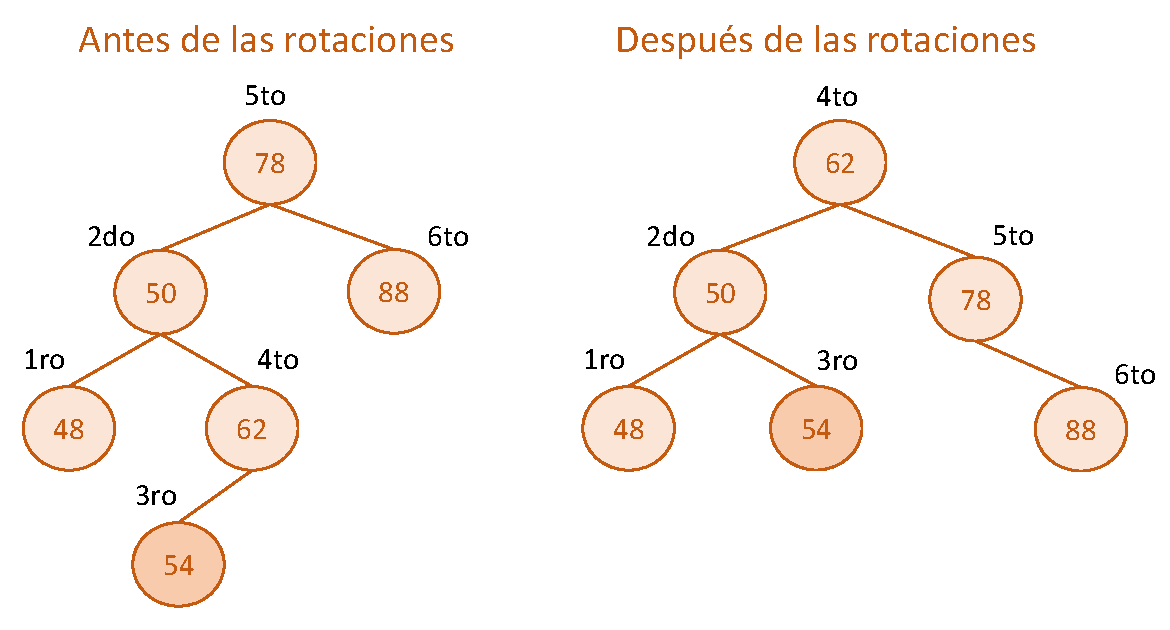
\includegraphics[scale=.42]{Graphics/AVL_rotations.pdf}
  	\caption{Las rotaciones preservan el entreorden.}\label{fig:AVL_rotations}
  \end{figure}

  Para obtener el nodo que posee índice $ i $ ($ i \geq 0 $) en el recorrido 
  entreorden de un ABB, se utiliza el método \textsc{Select} \cite[pág. 304]{MIT2}. 
  Este método no consulta el valor de los nodos que visita, sino la propiedad $ size[x] 
  $, que contiene el número de elementos del subárbol del cual $ x $ es raíz. Nótese que
  un nodo del ABB es determinado unívocamente por su lugar en el recorrido entreorden
  del árbol.
  
  Por ejemplo, siendo $ T $ el árbol de la figura \ref{fig:AVL_rotations}, para hallar el 
  tercer elemento del entreorden de $ T $, esto es, el elemento cuyo índice es 2 en dicho
  recorrido, se ejecuta \textsc{Select}($ root[T],\; 2 $), obteniendo como resultado el 
  nodo cuyo valor es 54.
  
  Otras operaciones del ABB que no requieren conocer el valor de sus nodos son
  \textsc{Tree-Minimum}, \textsc{Tree-Maximum} y \textsc{Tree-Successor} \cite[pág. 
  258-259]{MIT2}. \textsc{Tree-Minimum} y \textsc{Tree-Maximum} obtienen el elemento más a la 
  izquierda y el elemento más a la derecha de un ABB, respectivamente. En el caso de 
  \textsc{Tree-Successor}, su resultado es el sucesor de un nodo en el recorrido entreorden.
  
  Teniendo en cuenta lo anterior, en esta sección se presenta el \textbf{Á}rbol 
  \textbf{B}inario \textbf{B}alanceado (\textbf{BBT}, por sus siglas en inglés). Esta 
  estructura es un árbol binario balanceado por alturas, como el AVL, sólo que no es un 
  árbol de búsqueda, o sea, los valores de los elementos no guardan relación entre sí.
  Aunque no es un ABB, en el BBT es posible implementar las operaciones \textsc{Select},
  \textsc{Tree-Minimum}, \textsc{Tree-Maximum} y \textsc{Tree-Successor}, ya que estas no 
  requieren examinar el valor de los nodos del árbol \cite{MIT2}. En un BBT, también es 
  posible implementar las  rotaciones que se realizan en un AVL, ya que estas se limitan al 
  manejo de referencias y el conocimiento de la altura de cada subárbol, sin consultar el 
  valor de los nodos \cite{AVL}.
  
  \textbf{QuickList} es una estructura de datos que emplea el BBT para almacenar los
  elementos que posee. Es una lista que implementa las operaciones declaradas en la
  sección \ref{sec:oper}. La manera en que QuickList implementa cada una de estas 
  operaciones es descrita a continuación.
%-------------------------------------------------------------------------------------
\subsection{Get-At($ i $)}\label{subsec:qlGet}
%-------------------------------------------------------------------------------------
  El orden en que se encuentran los elementos de una QuickList corresponde al entreorden
  del BBT subyacente. Por esto, para obtener el $ i $-ésimo elemento, se utiliza el
  método \textsc{Select}.
  
  En el algoritmo \ref{algo:qlGet} se obtiene el nodo que ocupa la posición $ i $-ésima en
  el entreorden, llamando al método \textsc{Select} en la raíz del BBT $ T $. Luego se 
  devuelve el valor de dicho nodo, que se almacena en el campo $ key $.
  
  \begin{algorithm}[htb]\label{algo:qlGet}
  	\caption{QuickList \textsc{Get-At}}
  	
  	\SetAlgoLined
  	
  	\KwData{$i$}
  	\KwResult{$ i $-ésimo elemento de la lista.}
  	
  	\LinesNumbered
  	\SetAlgoVlined
  	
  	$ x \la $ \textsc{Select($root[T],\; i $)}\;
  	
  	\Return $ key[x] $\;
  \end{algorithm}

  El tiempo que consume el llamado a \textsc{Select} es, como mucho, proporcional a la
  altura del árbol $ T $ \cite[pág. 304]{MIT2}. Como $ T $ es un árbol balanceado, su 
  altura es $ O(\log n) $, donde $ n $ es el número de nodos. Por lo tanto, el tiempo de 
  corrida del \textsc{Select}, así como también del algoritmo \ref{algo:qlGet}, es $ 
  O(\log n) $.
%-------------------------------------------------------------------------------------
\subsection{Set-At($ i,\; c $)}\label{subsec:qlSet}
%-------------------------------------------------------------------------------------
  Para cambiar el valor de un nodo, basta con buscarlo en el BBT y colocar en el campo
  $ key $ el nuevo valor.
  
  En el algoritmo \ref{algo:qlSet} se obtiene el $ i $-ésimo nodo mediante el método
  \textsc{Select} y se actualiza el atributo $ key $ de dicho nodo con el nuevo valor.
  
  \begin{algorithm}[htb]\label{algo:qlSet}
  	\caption{QuickList \textsc{Set-At}}
  	
  	\SetAlgoLined
  	
  	\KwData{$i,\; c$}
  	
  	\LinesNumbered
  	\SetAlgoVlined
  	
  	$ x \la $\textsc{Select($root[T],\; i $)}\;
  	$key[x] \la c$\;
  \end{algorithm}

  El llamado a \textsc{Select} toma $ O(\log n) $, por tanto el algoritmo \ref{algo:qlSet}
  también.
%-------------------------------------------------------------------------------------
\subsection{Insert($ i,\; c $)}\label{subsec:qlInsert}
%-------------------------------------------------------------------------------------
  Sea $\; R = \langle d_0, d_1, ..., d_{n - 1} \rangle \;$ una ruta de $ n $ clientes. 
  Tras aplicar el método \textsc{Insert}($ i,\; c $) a $ R $, se obtiene la ruta
  $ R' = \langle d_0, d_1, ..., c, d_i, d_{i + 1}, ..., d_{n - 1} \rangle $. Luego de la
  inserción, $ c $ pasa a ser el antecesor del $ i $-ésimo cliente de $ R $, denotado
  como $ d_i $. En una QuickList esto se manifiesta de la siguiente forma: $ c $ pasa a ocupar 
  el puesto anterior a $\; d_i \;$ en el entreorden del BBT subyacente.
  
  Sea $ T $ el BBT correspondiente a una QuickList que contiene almacenados los clientes
  de $ R $. Sean $ x $ el nodo de $ T $ cuyo valor es $\; d_i \;$ e $\; y \;$ el nodo a 
  insertar, cuyo valor es $ c $. Si $ x $ no posee hijo izquierdo, entonces colocar a 
  $\; y \;$ como tal, garantiza que aparezca justo antes que $ x $ en el entreorden de $ T $.
  En otro caso, colocar a $\; y \;$ como elemento más a la derecha del subárbol del hijo 
  izquierdo de $ x $, lo hace aparecer como antecesor de $ x $ en el entreorden.
  
  En la figura \ref{fig:BBT_inserting} se muestran estos dos casos, así como el algoritmo para
  obtener el recorrido entreorden \cite[pág. 255]{MIT2}.
  
  \begin{figure}[htb]
  	\centering
  	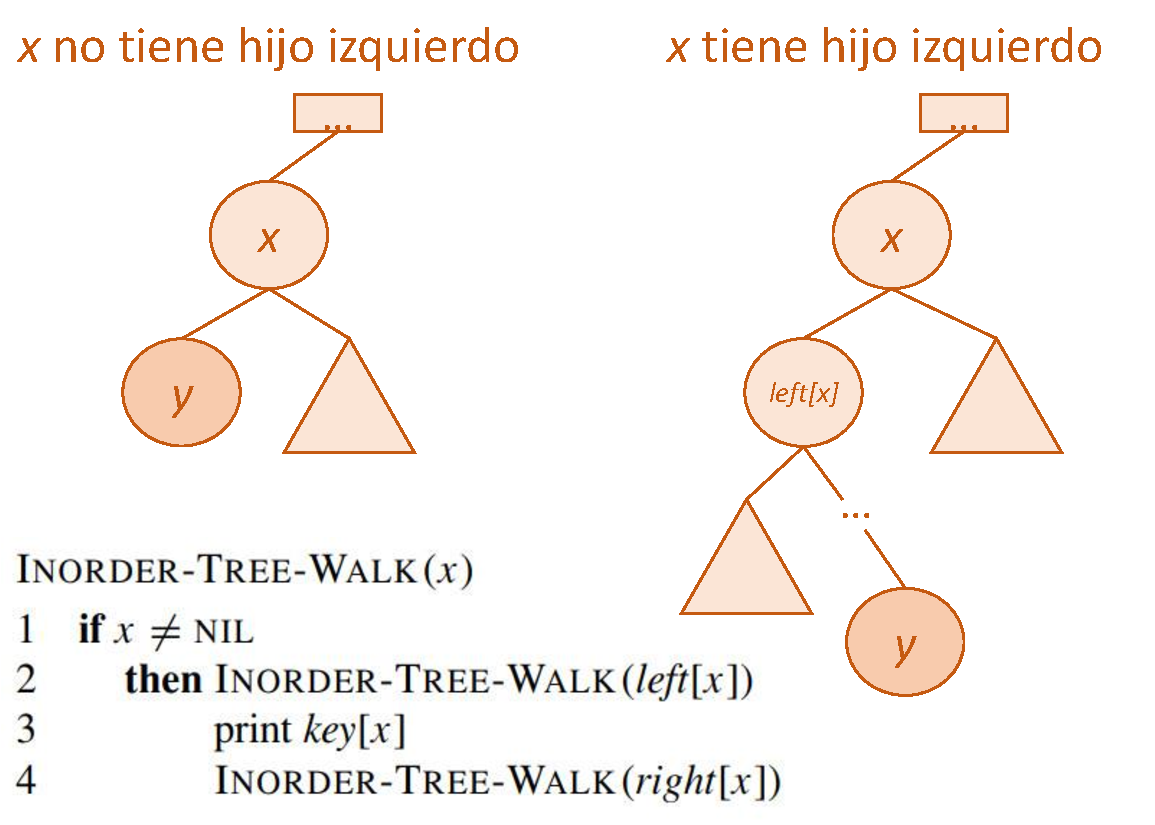
\includegraphics[scale=.45]{Graphics/BBT_inserting.pdf}
  	\caption{Colocando a $ y $ como antecesor de $ x $ en el entreorden.} \label{fig:BBT_inserting}
  \end{figure}

  Según el algoritmo \textsc{Inorder-Tree-Walk} de la figura \ref{fig:BBT_inserting}, primero 
  se obtiene el entreorden del subárbol izquierdo de $ x $ y luego el valor de este nodo. 
  Tenga $ x $ hijo izquierdo o no, el nodo $\; y \;$ es el elemento más a la derecha del 
  subárbol izquierdo de $ x $, tras la inserción. Por lo tanto, $\; y \;$ es el último 
  elemento del entreorden del árbol de $ left[x] $ y, en consecuencia, el antecesor de $ x $ 
  en dicho recorrido.
  
  En el algoritmo \ref{algo:qlInsert} se implementa esta idea. Si $ i = n $, entonces $ c $
  debe ser insertado al final de la ruta, por lo tanto, se coloca a $\; y \;$ como elemento más
  a la derecha del BBT $ T $. Para esto, $\; y \;$ pasa a ser el hijo derecho del último 
  elemento del entreorden de $ T $, el cual se obtiene mediante un llamado a 
  \textsc{Tree-Maximum}. En otro caso, esto es, si $\; 0 \leq i < n $, entonces se coloca a 
  $\; y \;$ como antecesor del $ i $-ésimo nodo en el entreorden, tal y como se explicó 
  anteriormente.
  
  Una vez insertado el nodo $\; y $, se procede a balancear la estructura, para mantener
  la invariante del BBT.
  
  \begin{algorithm}[htb]\label{algo:qlInsert}
  	\caption{QuickList \textsc{Insert}}
  	
  	\SetAlgoLined
  	
  	\KwData{$i, \;c$}
  	
  	\LinesNumbered
  	\SetAlgoVlined
  	
  	$ y \la $ nuevo nodo de BBT\;
  	$ key[y] \la c $\;
  	\If{$ i = n $}{
  		$ M \la $ \textsc{Tree-Maximum($ root[T] $)}\;
  		$ right[M] \la y $\;
  	}
  	\Else{
  		$ x \la $ \textsc{Select($ root[T],\; i $)} \;
  		\If{$ left[x] \neq $ \textsc{NIL}}{
  			$ m \la $ \textsc{Tree-Maximum($ left[x] $)}\;
  			$ right[m] \la y $\;
  		}
  		\Else{
  			$ left[x] \la y $\;
  		}
  	}
  	balancear $ T $\;
  	
  \end{algorithm}
  
  El algoritmo \textsc{Tree-Maximum} se ejecuta en tiempo $ O(h) $ en un árbol de altura 
  $ h $ \cite[pág. 258]{MIT2}. En un BBT la altura es logarítmica con respecto a la cantidad 
  de nodos $ n $, por tanto, \textsc{Tree-Maximum} es $ O(\log n) $. De igual manera ocurre 
  con el método \textsc{Select}. En el caso de balancear la estructura mediante el empleo de
  rotaciones, el procedimiento es igualmente proporcional a la altura del árbol \cite{AVL}.
  Por todo esto, y aplicando \textit{Regla de la Suma}, el algoritmo \ref{algo:qlInsert} 
  es $ O(\log n) $.
%-------------------------------------------------------------------------------------
\subsection{Remove-At($ i $)}\label{subsec:qlRemove}
%-------------------------------------------------------------------------------------
  Para eliminar el $ i $-ésimo elemento de una QuickList, se emplea el método
  \textsc{Tree-Delete} \cite[pág. 262]{MIT2} sobre el BBT subyacente. Este algoritmo elimina
  un nodo de un ABB, sin embargo, en su ejecución no compara valores de los nodos, por lo 
  tanto, es perfectamente aplicable a un BBT.
  
  En el algoritmo \ref{algo:qlRemove}, primero se selecciona el $ i $-ésimo nodo para luego
  eliminarlo mediante el llamado a \textsc{Tree-Delete}. Posteriormente, se procede a
  balancear la estructura para mantener la invariante del BBT.
  
  \begin{algorithm}[htb]\label{algo:qlRemove}
  	\caption{QuickList \textsc{Remove-At}}
  	
  	\SetAlgoLined
  	
  	\KwData{$i$}
  	
  	\LinesNumbered
  	\SetAlgoVlined
  	
  	$ c \la $ \textsc{Select}($ root[T],\; i $)\;
  	\textsc{Tree-Delete}($ T,\; c $)\;
  	balancear $ T $\;
  	
  \end{algorithm}

  Tanto \textsc{Select} como \textsc{Tree-Delete} se ejecutan en tiempo $ O(h) $ en un árbol
  de altura $ h $ \cite[pág. 263]{MIT2}. Asimismo, balancear el BBT es $ O(h) $. De esta 
  manera, la ejecución del algoritmo \ref{algo:qlRemove} es $ O(\log n) $.

%------------------------------------------------------------------------------------
\subsection{Últimos apuntes}\label{subsec:qlSummary}
%------------------------------------------------------------------------------------
  Como se ha podido apreciar, la implementación que QuickList propone para cada una de las
  operaciones requeridas, posee complejidad temporal $ O(\log n) $, siendo $ n $ la cantidad
  de elementos de la estructura. Esto hace de QuickList una buena alternativa para almacenar
  los clientes de una ruta. Sin embargo, debido al empleo de rotaciones en los métodos
  \textsc{Insert} y \textsc{Remove-At} para mantener la invariante del BBT subyacente, estas
  operaciones poseen constantes asintóticas muy elevadas en su respectivos tiempos de 
  ejecución.
  
  En la próxima sección se presenta, igualmente, una variación de una estructura ya 
  conocida. Esta surge como una alternativa al uso de estructuras arbóreas como la 
  empleada en QuickList.
%------------------------------------------------------------------------------------
\section{Disordered Indexable Skip Lists}\label{sec:disli}
%------------------------------------------------------------------------------------
  \textit{Skip Lists} es una estructura de datos creada por William Pugh en 1989. La 
  simpleza de su implementación y la eficiencia de sus operaciones, han hecho de Skip Lists
  una buena sustituta para los árboles balanceados \cite{Pugh}. 
  
  Aunque las operaciones en un AVL son $ O(\log n) $ en el peor caso, y en Skip Lists son $ 
  O(\log n) $ con alta probabilidad, esta última posee una menor constante asintótica, 
  debido a que las rotaciones que se deben realizar a un AVL, luego de cada inserción 
  o eliminación, influyen negativamente en su eficiencia.
  
  El factor constante de un algoritmo juega un papel importante en su aplicación práctica,
  sobre todo si se trata de un algoritmo sub-linear. Por ejemplo, si dos algoritmos $ A $ y
  $ B $ tardan $ O(\log n) $ en procesar una consulta y $ B $ es dos veces más rápido que 
  $ A $, entonces en el tiempo que $ A $ procesa una consulta en un conjunto de $ n $ 
  elementos, $ B $ puede procesar una consulta en un conjunto de $ n^2 $ elementos 
  \cite{Pugh}.
  
  Por eso, en esta sección se presenta una modificación de Skip Lists, denominada 
  \textbf{DISLI}, acrónimo en inglés para \textbf{S}kip \textbf{Li}sts \textbf{D}esordenada 
  \textbf{I}ndexable. DISLI constituye una alternativa a QuickList, como Skip Lists a los 
  árboles balanceados.
  
  En [cita a wikipedia] se propone una modificación a Skip Lists para obtener el índice
  de cada elemento. Esta consiste en asignar un ``peso'' a cada una de las referencias entre
  nodos. 
  
  Sean $ x $ e $ y $ nodos del nivel $ i $, de forma tal que $ y $ es el nodo siguiente a
  $ x $ en ese nivel, o sea, $ y = x . \fwdi $ \footnote{En esta sección los 
  índices tienen como valor mínimo 1, para que exista congruencia con la bibliografía 
  empleada.}, entonces el \textbf{peso o anchura} de la referencia de $ x $ a $ y $, denotado 
  como $ w(x, y) $, se define
  \begin{equation}\label{eq:xWeight}
  	w_i(x, y) = \left\{ \begin{array}{ll}
						  \idx(y) - \idx(x) & \text{si } y \neq \text{NIL}\\
						  0               & \text{si } y = \text{NIL}
					  \end{array} \right.,
  \end{equation}
  donde $ \idx(x) $ expresa el índice que posee $ x $ en la estructura. El valor de $ w_i(x, y) $ queda contenido en el atributo $ \withi $ del nodo $ x $, denotado como $ x . \withi $. Para que \ref{eq:xWeight} se cumpla en caso de $ x = header $, se adopta como convenio $ \idx(header) = \disliHeaderIdxColor{-1} $.
  
  En la figura \ref{fig:idxSkipL} se muestra una Skip Lists con esta modificación, conocida como Skip Lists indexable. En el interior de cada nodo se encuentra su \disliNodeKeyColor{llave} y debajo, el \disliNodeIdxColor{índice} que posee, mientras que encima de cada referencia del nivel 2 o superior, se encuentra su peso. Con respecto a las referencias del nivel 1 se omite su peso por conveniencia. En \disliNilReferenceColor{gris} se encuentran las referencias a NIL, las cuales poseen peso \disliNilReferenceColor{0}.
  
  \begin{figure}[htb]
  	\centering
  	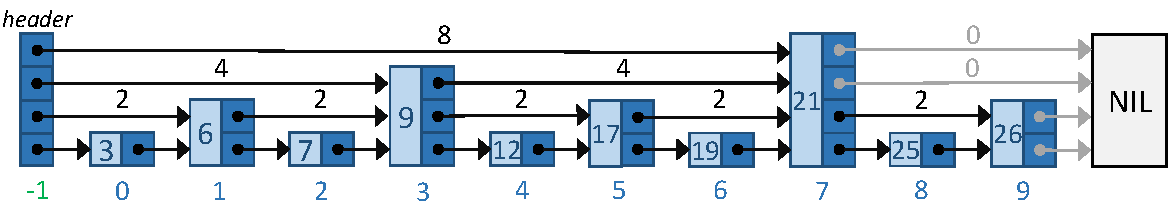
\includegraphics[scale=.51]{Graphics/Indexable_Skip_Lists.pdf}
  	\caption{Skip Lists indexable.}\label{fig:idxSkipL}
  \end{figure}

  Por ejemplo, si $ x $ es el nodo cuya llave es 9, entonces 
  $ x . \withT = \{1, 2, 4\}, $ ya que las referencias a los nodos de llaves 12, 17 y 21 poseen peso 1, 2 y 4, respectivamente.
  
  Los métodos \textsc{Insert} y \textsc{Delete} de una Skip Lists poseen una estructura similar \cite{Pugh}, dividiéndose en dos pasos fundamentales:
  \begin{enumerate}
  	\item[P1] Obtener en cada nivel el antecesor del elemento a insertar o eliminar.
  	\item[P2] Realizar los ajustes pertinentes según la operación en cuestión.
  \end{enumerate}

  Sea $ y $ el nodo a insertar o eliminar y se denota a su nodo antecesor en el nivel $ i $ como $ \predi(y) $. Debido a que en una Skip Lists usualmente los nodos se encuentran ordenados de forma creciente con respecto al atributo $ \key $, entonces una definición válida para 
  $ \predi(y) $ es
  \begin{equation}\label{eq:prediKeyDef}
	  \predi(y) = \underset{x . \key}{\max} \{ x : x . \key < y . \key \; \wedge \; x . \lev \geq i\} ,
  \end{equation}
  esto es, de todos los nodos con llave menor que $ y . \key $ y que se encuentra en el nivel $ i $-ésimo, el que mayor llave posea.
  
  En una Skip Lists indexable se puede obtener otra definición equivalente:
  \begin{equation}\label{eq:prediIdxDef}
	  \predi(y) = \underset{\idx(x)}{\max} \{ x : \idx(x) < \idx(y) \; \wedge \; x . \lev \geq i \} ,
  \end{equation}
  que obtiene, de los nodos inferiores a $ y $ en índice que se encuentran en el nivel $ i $, el que mayor índice posee. Esta definición, a diferencia de la anterior, no consulta el atributo $ \key $ de ningún nodo, por lo que puede ser perfectamente aplicable si los elementos de la estructura no mantienen un orden con respecto a esta propiedad.
  
  Así sucede en DISLI, que no es más que una Skip Lists indexable donde los valores del atributo $ \key $ no siguen ningún orden. DISLI satisface P1 mediante el método \textsc{Mark} (descrito a continuación), empleando las ecuaciones (\ref{eq:xWeight}) y (\ref{eq:prediIdxDef}). En el caso de P2 se procede de manera similar a una Skip Lists simple, sólo que algunos ajustes son pertinentes para mantener (\ref{eq:xWeight}) invariante.
  
  El método \textsc{Mark}$ (i) $ devuelve los antecesores, en todos los niveles, del $ i $-ésimo nodo, según la definición (\ref{eq:prediIdxDef}), así como el índice de cada uno de ellos. Para esto, se empieza en $ header $ en el nivel máximo de la lista, denotado por $ ListLevel $. Se recorre la lista enlazada de ese nivel de izquierda a derecha. En cada paso sobre un nodo $ x $, se garantiza que $ \idx(x) < i $. 
  
  Siendo $ y $ el nodo siguiente a $ x $ en la lista de ese nivel, si $ y $ es distinto de NIL, se halla su índice despejando en (\ref{eq:xWeight})
  \[ \idx(y) = \idx(x) + w(x, y). \]
  Si $ \idx(y) < i $, entonces $ x $ no es el antecesor del $ i $-ésimo nodo, porque $ \idx(x) < \idx(y) < i $, por lo tanto, se continúa iterando en ese nivel. En caso contrario, $ x $ es el antecesor buscado, ya que $ \idx(x) < i $ y no existe un nodo mayor que $ x $ en índice que cumpla esa propiedad, por lo tanto, se desciende un nivel y se repite el proceso, pero esta vez comenzando en $ x $. Una vez hallado el antecesor en el nivel 1, se detiene el algoritmo.
  
  Si $ y = $ NIL, entonces no hay nodos después de $ x $ en ese nivel, por lo tanto, $ x $ es el antecesor en dicho nivel del $ i $-ésimo elemento, y se procede como en el caso anterior.
  
  \begin{algorithm}[htb]\label{algo:disliMark}
  	\caption{\textsc{Mark}}
  	
  	\SetAlgoLined
  	
  	\KwData{$ i $}
  	
  	\LinesNumbered
  	\SetAlgoVlined
  	
  	$ update \la $ arreglo de tuplas $ \langle $nodo, índice$ \rangle $ de tamaño $ ListLevel $\;
  	$ x \la header$\;
  	$ idxX \la -1 $\;
  	$ level \la ListLevel $\;
  	
    \While{$ level \geq 1 $}{
    	$ y \la x . \fwd{level} $\;
    	\If{$ y \neq \nil \; \wedge \; idxX + w(x, y) < i $}{
    		$ idxX \la idxX + w(x, y) $\;
    		$ x \la y $\;
    	} \Else{
    		$ update[level] \la \langle x, \; idxX \rangle $\;
    		$ level \la level - 1 $\;
    	}
    }
    \Return $ update $\;
  \end{algorithm}
  
  El resultado del algoritmo \ref{algo:disliMark} es un arreglo que en cada posición almacena una tupla $ \langle $nodo, índice$\rangle$, que contiene el antecesor, y su índice, del $ i $-ésimo nodo de la lista, en el nivel que corresponde a dicha posición.
  
  A grandes rasgos, la única diferencia entre \textsc{Mark} y la propuesta de \cite{Pugh} para satisfacer P1, es el criterio aplicado a cada nodo para determinar si es o no el antecesor buscado. Uno emplea la definición (\ref{eq:prediIdxDef}), mientras que el otro, la (\ref{eq:prediKeyDef}). Dejando esto a un lado, ambos algoritmos tienen comportamientos idénticos, siendo la manera en que recorren la estructura el que más sobresale. 
  
  En la figura \ref{fig:mark5} se muestra el recorrido realizado por el algoritmo \textsc{Mark}, donde $ i = 5 $.
  \begin{figure}[htb]
  	\centering
  	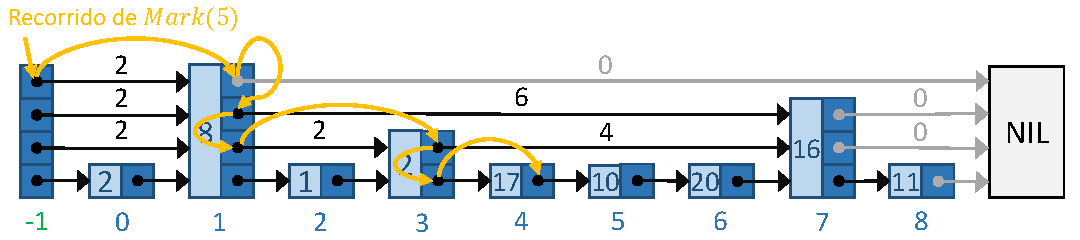
\includegraphics[scale=.56]{Graphics/DISLI_Mark(5).pdf}
  	\caption{Recorrido realizado en una DISLI por el llamado a \textsc{Mark}(5).}\label{fig:mark5}
  \end{figure}
  
  Por todo esto, el análisis de la complejidad temporal del algoritmo \ref{algo:disliMark} y el propuesto en \cite{Pugh}, es el mismo, resultando, con alta probabilidad, en una cota superior logarítmica con respecto al tamaño de la entrada.
  
  Hasta ahora, se presentó la Skip Lists Desordenada Indexable y su método \textsc{Mark}. A continuación se presenta la implementación que DISLI propone para cada una de las operaciones \textsc{Get-At, Set-At, Insert} y \textsc{Remove-At}, en las cuales el algoritmo \ref{algo:disliMark} juega un papel fundamental.
  
%-------------------------------------------------------------------------------------
\subsection{Get-At($ i $)}\label{subsec:disliGet}
%-------------------------------------------------------------------------------------
  Para implementar el método \textsc{Get-At}, se obtiene el antecesor del $ i $-ésimo nodo en el nivel 1, mediante el método \textsc{Mark}, y luego se accede a su llave mediante el atributo $ \key $.
  \begin{algorithm}[htb]\label{algo:disliGetAt}
  	\caption{DISLI \textsc{Get-At}}
  	
  	\SetAlgoLined
  	
  	\KwData{$ i $}
  	
  	\LinesNumbered
  	\SetAlgoVlined
  	
  	$ update \la $ \textsc{Mark}$ (i) $\;
  	$ \langle pred, \; idx \rangle \la update[1] $\;
  	$ x \la pred . \fwd{1} $\;
  	\Return $ x . \key $\;
  \end{algorithm}

  El mayor peso del costo temporal de este algoritmo recae en el llamado a \textsc{Mark}, y este toma $ O(\log n) $ con alta probabilidad, siendo $ n $ la cantidad de elementos de la lista. Por esto, el algoritmo \ref{algo:disliGetAt} se comporta de igual manera.
  
%-------------------------------------------------------------------------------------
\subsection{Set-At($ i,\; c $)}\label{subsec:disliSet}
%-------------------------------------------------------------------------------------
  Para implementar esta operación, se obtiene el $ i $-ésimo nodo de la estructura, como se procedió en la operación anterior, y se modifica su llave. El algoritmo \ref{algo:disliSet} describe este proceso.
  \begin{algorithm}[htb]\label{algo:disliSet}
  	\caption{DISLI \textsc{Set-At}}
  	
  	\SetAlgoLined
  	
  	\KwData{$ i, \; c $}
  	
  	\LinesNumbered
  	\SetAlgoVlined
  	
  	$ update \la $ \textsc{Mark}$ (i) $\;
  	$ \langle pred, \; idx \rangle \la update[1] $\;
  	$ x \la pred . \fwd{1} $\;
  	$ x . \key \la c $\;
  \end{algorithm}

  Resulta poco probable que el método \textsc{Mark}  no posea orden logarítmico, por tanto, el algoritmo \ref{algo:disliSet} es $ O(\log n) $ con alta probabilidad.
  
%-------------------------------------------------------------------------------------
\subsection{Insert($ i,\; c $)}\label{subsec:disliInsert}
%-------------------------------------------------------------------------------------
  Cuando se inserta un nuevo elemento, se crea un nodo $ x $ en la DISLI y se le asigna un nivel aleatorio \cite{Pugh}. El nuevo nodo entonces gana altura y pasa a ocupar un lugar en la lista, aumentando el índice de aquellos elementos a su derecha. Por todo esto, además de crearse nuevas referencias, otras deben ser actualizadas. Estas son, precisamente, aquellas pertenecientes a los antecesores del $ i $-ésimo nodo, en cada uno de los niveles. 
  
  Sean $ y $ el $ i $-ésimo nodo de la lista antes de insertar a $ x, \; z = \pred{j}(y) $. Si $ j \leq x . \lev $, entonces, tras la inserción, $ x $ pasa a ocupar un lugar a continuación de $ z $ en la lista enlazada del nivel $ j $ y, en consecuencia, nuevas referencias deben ser creadas, asignándoles a cada una el peso correspondiente. De lo contrario, la referencia de $ z $ hacia su sucesor en el nivel $ j $ no cambia, sin embargo, si no apunta a NIL, aumenta su peso en una unidad, debido a que el índice de $ z . \fwd{j} $ se incrementa en la misma medida, producto de la inserción de $ x $.
  
  La figura \ref{fig:disliInsertion} ilustra este proceso, mostrando la inserción del elemento 13 en la quinta posición de una DISLI, donde se le asigna nivel 2 al nuevo nodo. En {\red rojo} se muestran las referencias que se ``dividen en dos'' producto de la inserción del nuevo elemento, mientras que en \disliWUpRef{verde}, aquella que sólo ganó peso.
  \begin{figure}[htb]
  	\hspace{-1.5cm}
  	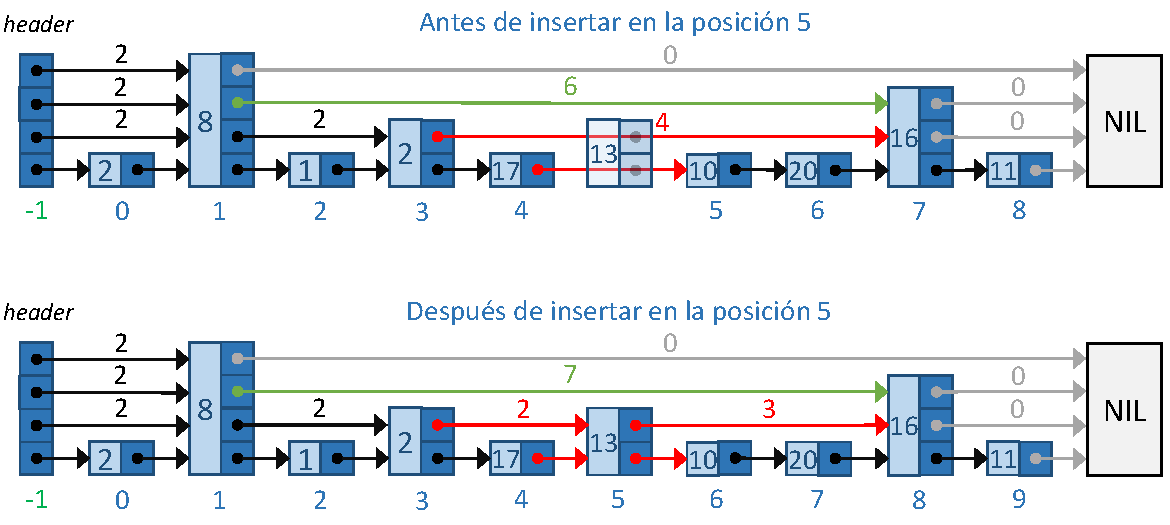
\includegraphics[scale=.5]{Graphics/DISLI_insertion.pdf}
  	\caption{Inserción en una DISLI del elemento 13 en la posición 5.}\label{fig:disliInsertion}
  \end{figure}

  En el algoritmo \ref{algo:disliInsert}, se obtienen todos los antecesores del $ i $-ésimo nodo mediante un llamado al método \textsc{Mark}. Luego, se crea el nuevo nodo $ x $, se le asigna un nivel aleatorio mediante el método \textsc{randomLevel} de \cite{Pugh} y se establece a $ c $ como su llave. Si el nivel escogido para $ x $ supera al nivel máximo de la DISLI, entonces se coloca a $ header $ como su antecesor en los niveles superiores a $ ListLevel $. Posteriormente, se procede a insertar a $ x $ en las listas enlazadas de los niveles iguales o inferiores a $ x.\lev $, realizando los cambios correspondientes a las referencias y la función $ w $. En el caso de los restantes niveles, si la referencia de $ z $ no apunta a NIL, se realiza el incremento de su peso.
  \begin{algorithm}[htb]\label{algo:disliInsert}
  	\caption{DISLI \textsc{Insert}}
  	
  	\SetAlgoLined
  	
  	\KwData{$ i, \; c $}
  	
  	\LinesNumbered
  	\SetAlgoVlined
  	
  	$ update \la $ \textsc{Mark}($ i $)\;
  	$ x \la $ nuevo nodo de DISLI\;
  	$ x . \lev \la $ \textsc{randomLevel}()\;
  	$ x . \key \la c $\;
  	\If{$ x . \lev > ListLevel $}{
  		\For{$ j \la ListLevel + 1 $ {\bf to} $ x . \lev $}{
  			$ update[j] \la \langle header, \; -1 \rangle $\;
  			$ header . \fwd{j} \la \nil $\;
  			$ header . \with{j} \la 0 $\;
  			
  		}
  		$ ListLevel \la x . \lev $\;
  	}
    \For{$ j \la 1 $ {\bf to} $ x . \lev $}{
    	$ \langle z, \; idxZ \rangle \la update[j] $\;
    	$ x . \fwd{j} \la z . \fwd{j} $\;
    	$ z . \fwd{j} \la x $\;
    	\If{$ x.\fwd{j} = \nil $}{
    		$ x.\with{j} \la 0 $\;
    	} \Else{
    		$ x . \with{j} \la z . \with{j} - i + idxZ + 1 $\;
    	}
    	$ z . \with{j} \la i - idxZ $\;
    }
	\For{$ j \la x . \lev + 1 $ {\bf to} $ ListLevel $}{
		$ \langle z, \; idxZ \rangle \la update[j] $\;
		\If{$ z . \fwd{j} \neq \nil $}{
			$ z . \with{j} \la z . \with{j} + 1 $\;
		}
	}
  \end{algorithm}

  Este algoritmo es una adaptación del método \textsc{Insert} presentado en \cite{Pugh}. La idea es muy similar, sólo que un poco de código extra es necesario para actualizar el atributo \withT, propio de DISLI.
  
  \textsc{Mark} es $ O(\log n) $ con alta probabilidad y el resto del algoritmo es $ O(x.\lev + ListLevel) $, por regla de la suma. La probabilidad de que el nivel máximo en una Skip Lists de $ n $ elementos sea significativamente mayor que $ \log_{1 / p} n $ es muy baja, siendo $ p \in (0, 1) $ un parámetro de la estructura \cite{Pugh}. Por todo esto, el algoritmo \ref{algo:disliInsert} es $ O(\log n) $ con alta probabilidad.
%-------------------------------------------------------------------------------------
\subsection{Remove-At($ i $)}\label{subsec:disliRemove}
%-------------------------------------------------------------------------------------
  Remover el $ i $-ésimo elemento de una DISLI es una operación muy similar a revertir un proceso de inserción en la misma posición. Para ello, se obtiene el antecesor del nodo a eliminar en cada uno de los niveles y se realizan los ajustes pertinentes en sus referencias.
  
  El algoritmo \ref{algo:disliRemove} implementa esta idea. Sean $ x $ el $ i $-ésimo nodo, $ z = \pred{j}(x) $ e $ y = z.\fwd{j} $. Si $ y = \nil $, entonces $ \forall k \geq j $ se cumple que $ \pred{k}(x).\fwd{k} = \nil $, por tanto las referencias de los antecesores de los niveles $ j $ y superiores no necesitan ser modificadas.
  
  Por otro lado, si $ x \neq y $, entonces $ \idx(x) < \idx(y) $, por tanto $ w(z, y) $ disminuye en una unidad, debido a que $ \idx(y) $ le sucede lo mismo, una vez $ x $ deja de pertenecer a la estructura. De lo contrario, se elimina a $ x $ de la lista enlazada del $ j $-ésimo nivel, actualizando el valor de $ z.\with{j} $.
  
  Luego, se actualiza el valor de $ ListLevel $ al nivel más alto donde se encuentra una lista enlazada no vacía.
  \begin{algorithm}[htb]\label{algo:disliRemove}
  	\caption{DISLI \textsc{Remove-At}}
  	
  	\SetAlgoLined
  	
  	\KwData{$ i $}
  	
  	\LinesNumbered
  	\SetAlgoVlined
  	
  	$ update \la $ \textsc{Mark}($ i $)\;
  	$ \langle z_1, \; idxZ_1 \rangle \la update[1] $\;
  	$ x \la z_1.\fwd{1} $\;
  	\For{$ j \la 1 \; \To \; ListLevel $}{
  		$ \langle z, \; idxZ \rangle \la update[j] $\;
  		\If{$ z.\fwd{j} = \nil $}{
  			{\bf break}\;
  		}
  		\If{$ z.\fwd{j} \neq x $}{
  			$ z.\with{j} \la z.\with{j} - 1 $\;
  		} \Else{
  			$ z.\fwd{j} \la x.\fwd{j} $\;
  			\If{$ z.\fwd{j} \neq \nil $}{
  				$ z.\with{j} \la z.\with{j} + x.\with{j} - 1 $\;
  			} \Else{
  				$ z.\with{j} \la 0 $
  			}
  		}
  	}
    destruir nodo $ x $\;
    \While{$ ListLevel > 1 \; \wedge \; header.\fwd{ListLevel} = \nil $}{
    	$ ListLevel \la ListLevel - 1 $\;
    }
  \end{algorithm}

  El llamado a \textsc{Mark} es $ O(\log n) $ con alta probabilidad. El resto del algoritmo \ref{algo:disliRemove} es $ O(ListLevel) $, que es altamente probable que sea $ O(\log n) $. Por todo esto, el algoritmo anterior posee orden logarítmico.
  
%------------------------------------------------------------------------------------
\subsection{Últimos apuntes}\label{subsec:disliSummary}
%------------------------------------------------------------------------------------
  En esta sección fue presentada la Skip Lists Desordenada Indexable, una variante de Skip Lists donde las llaves de los nodos no están sujetas a criterio de ordenación alguno. Esta estructura de datos implementa eficientemente, con alta probabilidad, las operaciones requeridas por el algoritmo IVNS presentado en \cite{Andy}.
  
  En la sección \ref{sec:resul} se exponen los resultados obtenidos por el empleo de QuickList y DISLI en el algoritmo mencionado. En el caso de DISLI, se utilizan diversos valores de $ p $, una constante empleada en el método \textsc{randomLevel} para obtener aleatoriamente los niveles de los nodos a insertar en la estructura \cite{Pugh}. La alteración del valor de $ p $ influye en el comportamiento de DISLI y esto repercute en los resultados que se obtienen.
  
%===================================================================================

%===================================================================================
% Resultados
%-----------------------------------------------------------------------------------
\section{Resultados}\label{sec:resul}
%===================================================================================

%===================================================================================
% Conclusiones
%-----------------------------------------------------------------------------------
\section{Conclusiones}\label{sec:conc}

  En esta sección puede incluir las conclusiones de su investigación y las ideas
  sobre la continuidad del trabajo, en el caso que aplique.

%===================================================================================

%===================================================================================
% Recomendaciones
%-----------------------------------------------------------------------------------
\section{Recomendaciones}\label{sec:rec}

  En esta sección puede incluir recomendaciones sobre posibles formas de continuar
  la investigación u otros temas relacionados.

%===================================================================================



%===================================================================================
% Bibliografía
%-----------------------------------------------------------------------------------
\begin{thebibliography}{99}
%-----------------------------------------------------------------------------------
	\bibitem{Camila} Pérez Mosquera, C. (2017).	\emph{Primeras aproximaciones 
	a la Búsqueda de Vecindad Infinitamente Variable}. $\;$ Facultad de Matemática y 
	Computación, Universidad de La Habana.
	
	\bibitem{Paolo} Paolo Toth; Daniele Vigo (2001) $\;$ \textit{The Vehicle Routing 
	Problem (Monographs on Discrete Mathematics and Applications)}. $\;$ Monographs on 
	Discrete Mathematics and Applications. SIAM $\;$ MIT Press.
	
	\bibitem{Andy} Ledesma García, Andy; Hernández Ramírez, Omar Alejandro. (2020) $\;$
	\textit{Búsqueda de Vecindad Infinitamente Variable con SAG}. $\;$ Facultad de
	Matemática y Computación, Universidad de La Habana.
	
	\bibitem{MIT2} Cormen, T. H.; Leiserson, Ch. E.; Rivest, R. L; Stein, C. (2002).
	$\;$ \textit{Introduction to Algorithms, Second Edition}. $\;$ McGraw-Hill Book 
	Company; The MIT Press.
	
	\bibitem{Alina}  Fernández Arias, Alina. $\;$ \textit{El problema de enrutamiento de 
	vehículos con recogida y entrega simultánea considerando una flota heterogénea.} 
	$\;$ Master’s thesis, Facultad de Matemática y Computación. Universidad de La Habana, 
	La Habana, Cuba, 7 2010.
	
	\bibitem{Mla} N Mladenovic. $\;$ \textit{A variable neighborhood algorithm - a new 
	metaheuristic for optimization combinatorial.}$\;$ In Abstract of papers presented at 
	Optimization Days, Montreal, volume 12, 1995.
	
	\bibitem{AVL} G. M. Adel’son-Vel’ski\u{\i} y E. M. Landis. $\;$
	\textit{An algorithm for the organization of information}.$\;$ Soviet Mathematics 
	Doklady, 3(5):1259–1263, 1962.
	
	\bibitem{Pugh} Pugh, William. $ \; $ \textit{Skip Lists: A Probabilistic Alternative to
	Balanced Trees.}

%-----------------------------------------------------------------------------------
\end{thebibliography}

%-----------------------------------------------------------------------------------

\label{end}

\end{document}

%===================================================================================
